\section{COMPLETUDE DOS DADOS}

\begin{figure}[htb!]
    \centering
	\captionsetup{justification=raggedright, singlelinecheck=false, width=1\textwidth}
    \caption{Gráfico de completude dos dados para o mês de setembro/2023 para as estações BCM2 e MC9.}
    \begin{mdframed}[
        linecolor=black,
        linewidth=1pt,
        roundcorner=10pt,
    ]
    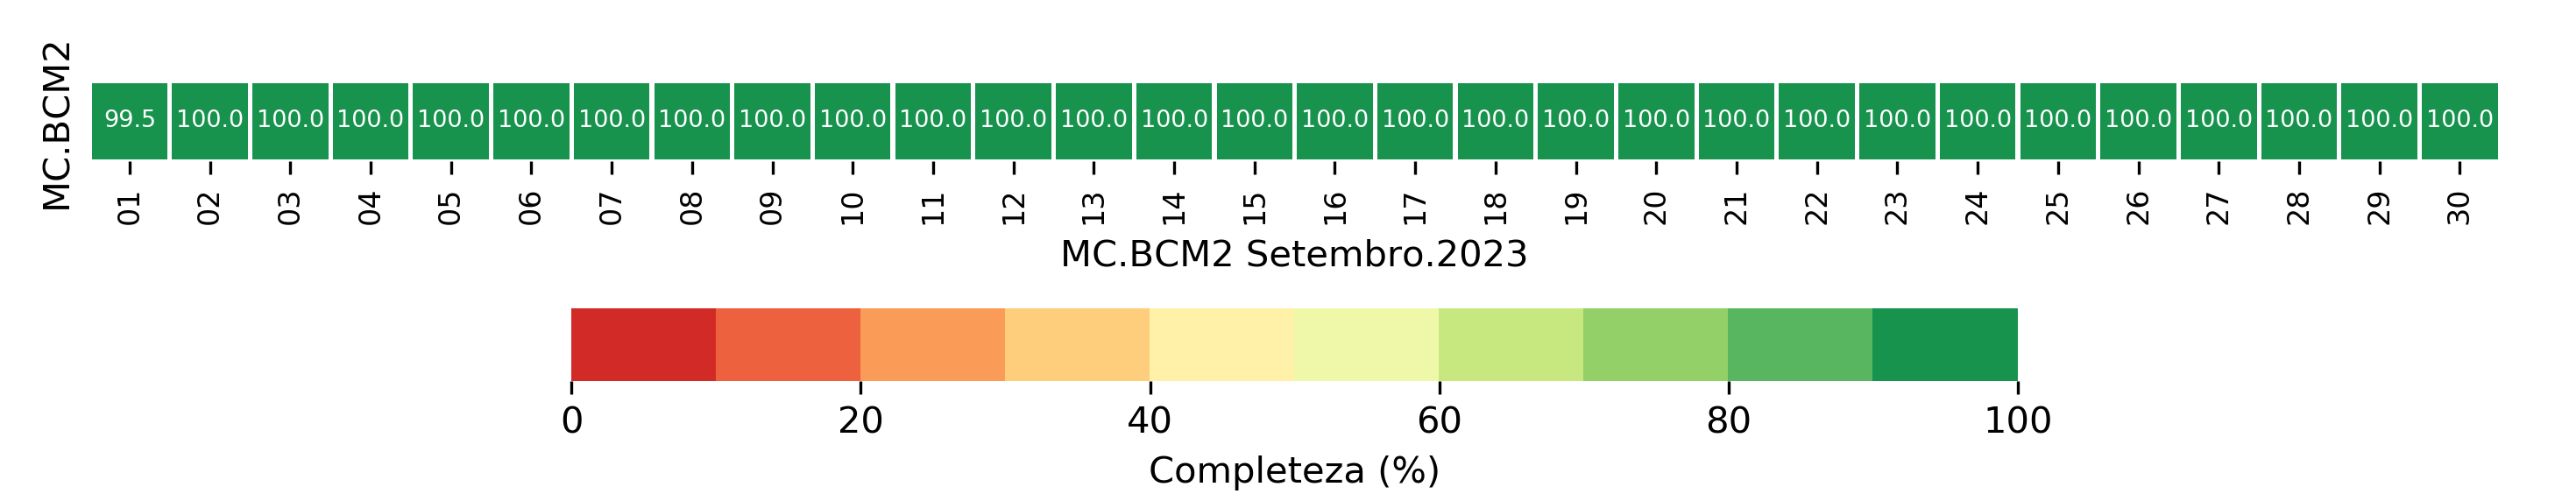
\includegraphics[width=1.0\textwidth]{./machadinho/figuras/completude_BCM2.png} % Substitua pelo nome da imagem e ajuste o tamanho
    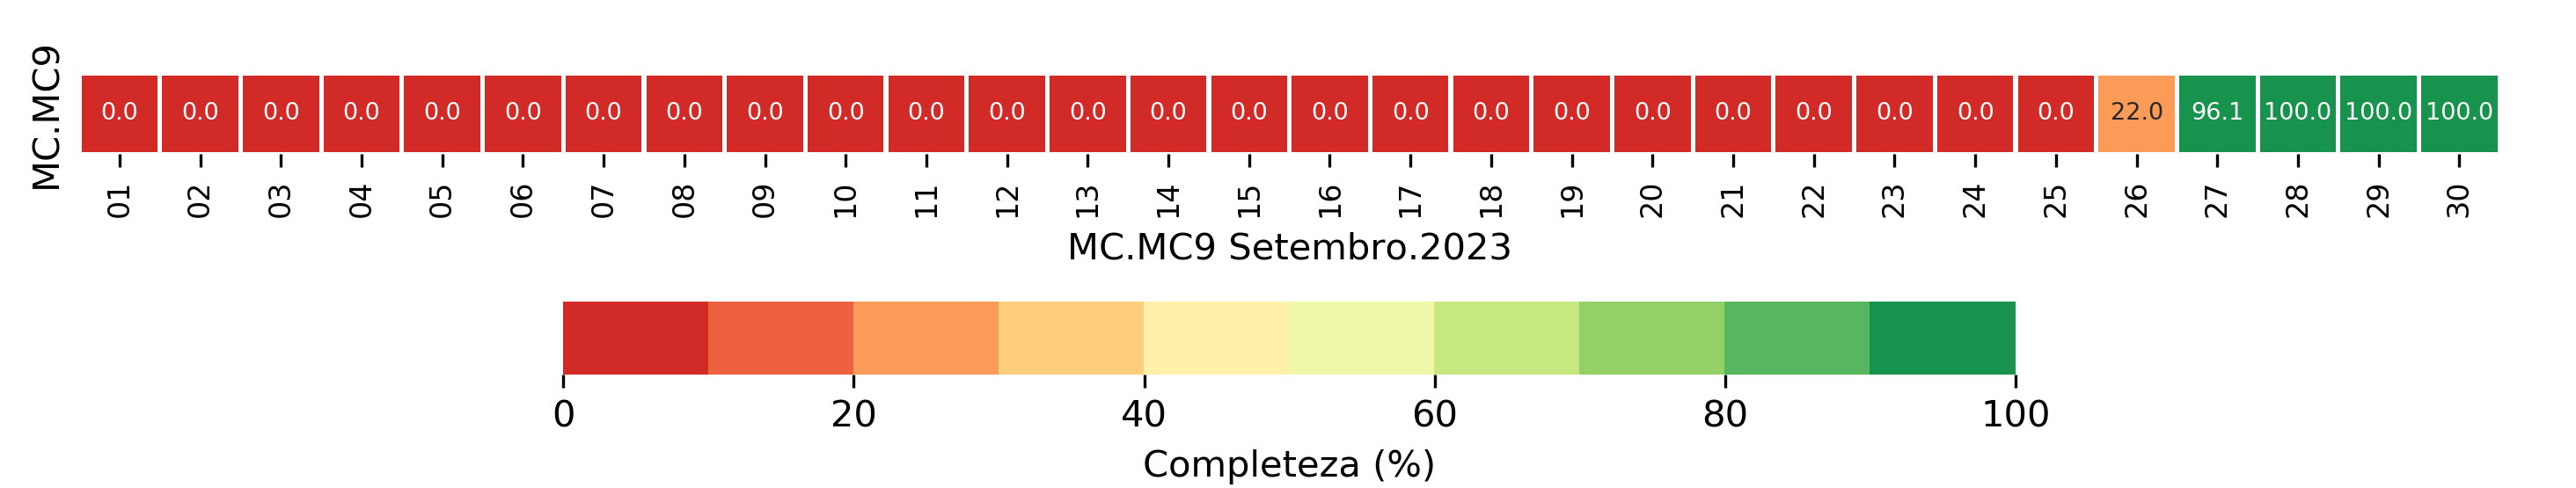
\includegraphics[width=1.0\textwidth]{./machadinho/figuras/completude_MC9.png}
    \end{mdframed}
    \caption*{Fonte: IPT}
    \label{fig:completude}
\end{figure}

